\documentclass[8pt]{beamer}

% Beamer style
%\usetheme[secheader]{Madrid}
% \usetheme{CambridgeUS}
\useoutertheme{infolines}
\usecolortheme[rgb={0.65,0.15,0.25}]{structure}
% \usefonttheme[onlymath]{serif}
\beamertemplatenavigationsymbolsempty
%\AtBeginSubsection

% Packages
%\usepackage[french]{babel}
\usepackage[latin1]{inputenc}
\usepackage{color}
% \usepackage[dvipsnames]{xcolor}
\usepackage{xspace}
\usepackage{dsfont, stmaryrd}
\usepackage{amsmath, amsfonts, amssymb, stmaryrd, mathabx}
\usepackage{epsfig}
\usepackage{tikz}
\usepackage{url}
% \usepackage{ulem}
\usepackage{/home/robin/LATEX/Biblio/astats}
%\usepackage[all]{xy}
\usepackage{graphicx}

% Maths
% \newtheorem{theorem}{Theorem}
% \newtheorem{definition}{Definition}
\newtheorem{proposition}{Proposition}
% \newtheorem{assumption}{Assumption}
% \newtheorem{algorithm}{Algorithm}
% \newtheorem{lemma}{Lemma}
% \newtheorem{remark}{Remark}
% \newtheorem{exercise}{Exercise}
% \newcommand{\propname}{Prop.}
% \newcommand{\proof}{\noindent{\sl Proof:}\quad}
% \newcommand{\eproof}{$\blacksquare$}

% \setcounter{secnumdepth}{3}
% \setcounter{tocdepth}{3}
\newcommand{\pref}[1]{\ref{#1} p.\pageref{#1}}
\newcommand{\qref}[1]{\eqref{#1} p.\pageref{#1}}

% Colors : http://latexcolor.com/
\definecolor{darkred}{rgb}{0.65,0.15,0.25}
\definecolor{darkgreen}{rgb}{0,0.4,0}
\definecolor{darkred}{rgb}{0.65,0.15,0.25}
\definecolor{amethyst}{rgb}{0.6, 0.4, 0.8}
\definecolor{asparagus}{rgb}{0.53, 0.66, 0.42}
\definecolor{applegreen}{rgb}{0.55, 0.71, 0.0}
\definecolor{awesome}{rgb}{1.0, 0.13, 0.32}
\definecolor{blue-green}{rgb}{0.0, 0.87, 0.87}
\definecolor{red-ggplot}{rgb}{0.52, 0.25, 0.23}
\definecolor{green-ggplot}{rgb}{0.42, 0.58, 0.00}
\definecolor{purple-ggplot}{rgb}{0.34, 0.21, 0.44}
\definecolor{blue-ggplot}{rgb}{0.00, 0.49, 0.51}

% Commands
\newcommand{\backupbegin}{
   \newcounter{finalframe}
   \setcounter{finalframe}{\value{framenumber}}
}
\newcommand{\backupend}{
   \setcounter{framenumber}{\value{finalframe}}
}
\newcommand{\emphase}[1]{\textcolor{darkred}{#1}}
\newcommand{\comment}[1]{\textcolor{gray}{#1}}
\newcommand{\paragraph}[1]{\textcolor{darkred}{#1}}
\newcommand{\refer}[1]{{\small{\textcolor{gray}{{\cite{#1}}}}}}
\newcommand{\Refer}[1]{{\small{\textcolor{gray}{{[#1]}}}}}
\newcommand{\goto}[1]{{\small{\textcolor{blue}{[\#\ref{#1}]}}}}
\renewcommand{\newblock}{}

\newcommand{\tabequation}[1]{{\medskip \centerline{#1} \medskip}}
% \renewcommand{\binom}[2]{{\left(\begin{array}{c} #1 \\ #2 \end{array}\right)}}

% Variables 
\newcommand{\Abf}{{\bf A}}
\newcommand{\Beta}{\text{B}}
\newcommand{\Bcal}{\mathcal{B}}
\newcommand{\Bias}{\xspace\mathbb B}
\newcommand{\Cor}{{\mathbb C}\text{or}}
\newcommand{\Cov}{{\mathbb C}\text{ov}}
\newcommand{\cl}{\text{\it c}\ell}
\newcommand{\Ccal}{\mathcal{C}}
\newcommand{\cst}{\text{cst}}
\newcommand{\Dcal}{\mathcal{D}}
\newcommand{\Ecal}{\mathcal{E}}
\newcommand{\Esp}{\xspace\mathbb E}
\newcommand{\Espt}{\widetilde{\Esp}}
\newcommand{\Covt}{\widetilde{\Cov}}
\newcommand{\Ibb}{\mathbb I}
\newcommand{\Fcal}{\mathcal{F}}
\newcommand{\Gcal}{\mathcal{G}}
\newcommand{\Gam}{\mathcal{G}\text{am}}
\newcommand{\Hcal}{\mathcal{H}}
\newcommand{\Jcal}{\mathcal{J}}
\newcommand{\Lcal}{\mathcal{L}}
\newcommand{\Mt}{\widetilde{M}}
\newcommand{\mt}{\widetilde{m}}
\newcommand{\Nbb}{\mathbb{N}}
\newcommand{\Mcal}{\mathcal{M}}
\newcommand{\Ncal}{\mathcal{N}}
\newcommand{\Ocal}{\mathcal{O}}
\newcommand{\pt}{\widetilde{p}}
\newcommand{\Pt}{\widetilde{P}}
\newcommand{\Pbb}{\mathbb{P}}
\newcommand{\Pcal}{\mathcal{P}}
\newcommand{\Qcal}{\mathcal{Q}}
\newcommand{\qt}{\widetilde{q}}
\newcommand{\Rbb}{\mathbb{R}}
\newcommand{\Sbb}{\mathbb{S}}
\newcommand{\Scal}{\mathcal{S}}
\newcommand{\st}{\widetilde{s}}
\newcommand{\St}{\widetilde{S}}
\newcommand{\Tcal}{\mathcal{T}}
\newcommand{\todo}{\textcolor{red}{TO DO}}
\newcommand{\Ucal}{\mathcal{U}}
\newcommand{\Un}{\math{1}}
\newcommand{\Vcal}{\mathcal{V}}
\newcommand{\Var}{\mathbb V}
\newcommand{\Vart}{\widetilde{\Var}}
\newcommand{\Zcal}{\mathcal{Z}}

% Symboles & notations
\newcommand\independent{\protect\mathpalette{\protect\independenT}{\perp}}\def\independenT#1#2{\mathrel{\rlap{$#1#2$}\mkern2mu{#1#2}}} 
\renewcommand{\d}{\text{\xspace d}}
\newcommand{\gv}{\mid}
\newcommand{\ggv}{\, \| \, }
% \newcommand{\diag}{\text{diag}}
\newcommand{\card}[1]{\text{card}\left(#1\right)}
\newcommand{\trace}[1]{\text{tr}\left(#1\right)}
\newcommand{\matr}[1]{\boldsymbol{#1}}
\newcommand{\matrbf}[1]{\mathbf{#1}}
\newcommand{\vect}[1]{\matr{#1}} %% un peu inutile
\newcommand{\vectbf}[1]{\matrbf{#1}} %% un peu inutile
\newcommand{\trans}{\intercal}
\newcommand{\transpose}[1]{\matr{#1}^\trans}
\newcommand{\crossprod}[2]{\transpose{#1} \matr{#2}}
\newcommand{\tcrossprod}[2]{\matr{#1} \transpose{#2}}
\newcommand{\matprod}[2]{\matr{#1} \matr{#2}}
\DeclareMathOperator*{\argmin}{arg\,min}
\DeclareMathOperator*{\argmax}{arg\,max}
\DeclareMathOperator{\sign}{sign}
\DeclareMathOperator{\tr}{tr}
\newcommand{\ra}{\emphase{$\rightarrow$} \xspace}

% Hadamard, Kronecker and vec operators
\DeclareMathOperator{\Diag}{Diag} % matrix diagonal
\DeclareMathOperator{\diag}{diag} % vector diagonal
\DeclareMathOperator{\mtov}{vec} % matrix to vector
\newcommand{\kro}{\otimes} % Kronecker product
\newcommand{\had}{\odot}   % Hadamard product

% TikZ
\newcommand{\nodesize}{2em}
\newcommand{\edgeunit}{2.5*\nodesize}
\newcommand{\edgewidth}{1pt}
\tikzstyle{node}=[draw, circle, fill=black, minimum width=.75\nodesize, inner sep=0]
\tikzstyle{square}=[rectangle, draw]
\tikzstyle{param}=[draw, rectangle, fill=gray!50, minimum width=\nodesize, minimum height=\nodesize, inner sep=0]
\tikzstyle{hidden}=[draw, circle, fill=gray!50, minimum width=\nodesize, inner sep=0]
\tikzstyle{hiddenred}=[draw, circle, color=red, fill=gray!50, minimum width=\nodesize, inner sep=0]
\tikzstyle{observed}=[draw, circle, minimum width=\nodesize, inner sep=0]
\tikzstyle{observedred}=[draw, circle, minimum width=\nodesize, color=red, inner sep=0]
\tikzstyle{eliminated}=[draw, circle, minimum width=\nodesize, color=gray!50, inner sep=0]
\tikzstyle{empty}=[draw, circle, minimum width=\nodesize, color=white, inner sep=0]
\tikzstyle{blank}=[color=white]
\tikzstyle{nocircle}=[minimum width=\nodesize, inner sep=0]

\tikzstyle{edge}=[-, line width=\edgewidth]
\tikzstyle{edgebendleft}=[-, >=latex, line width=\edgewidth, bend left]
\tikzstyle{edgebendright}=[-, >=latex, line width=\edgewidth, bend right]
\tikzstyle{lightedge}=[-, line width=\edgewidth, color=gray!50]
\tikzstyle{lightedgebendleft}=[-, >=latex, line width=\edgewidth, bend left, color=gray!50]
\tikzstyle{lightedgebendright}=[-, >=latex, line width=\edgewidth, bend right, color=gray!50]
\tikzstyle{edgered}=[-, line width=\edgewidth, color=red]
\tikzstyle{edgebendleftred}=[-, >=latex, line width=\edgewidth, bend left, color=red]
\tikzstyle{edgebendrightred}=[-, >=latex, line width=\edgewidth, bend right, color=red]

\tikzstyle{arrow}=[->, >=latex, line width=\edgewidth]
\tikzstyle{arrowbendleft}=[->, >=latex, line width=\edgewidth, bend left]
\tikzstyle{arrowbendright}=[->, >=latex, line width=\edgewidth, bend right]
\tikzstyle{arrowred}=[->, >=latex, line width=\edgewidth, color=red]
\tikzstyle{arrowbendleftred}=[->, >=latex, line width=\edgewidth, bend left, color=red]
\tikzstyle{arrowbendrightred}=[->, >=latex, line width=\edgewidth, bend right, color=red]
\tikzstyle{arrowblue}=[->, >=latex, line width=\edgewidth, color=blue]
\tikzstyle{dashedarrow}=[->, >=latex, dashed, line width=\edgewidth]
\tikzstyle{dashededge}=[-, >=latex, dashed, line width=\edgewidth]
\tikzstyle{dashededgebendleft}=[-, >=latex, dashed, line width=\edgewidth, bend left]
\tikzstyle{lightarrow}=[->, >=latex, line width=\edgewidth, color=gray!50]

\newcommand{\dN}{\Delta N}
\newcommand{\dtau}{\Delta \tau}

% Directory
\newcommand{\figcp}{/home/robin/RECHERCHE/RUPTURES/EXPOSES/FIGURES}

%====================================================================
%====================================================================

%====================================================================
%====================================================================
\begin{document}
%====================================================================
%====================================================================

%====================================================================
\title[Change-point in Poisson process]{Change-point detection in a Poisson process}

\author[S. Robin]{S. Robin \\ \medskip
joint ongoing work with E. Lebarbier, C. Dion-Blanc}

\institute[]{Sorbonne universit�}

\date[Rochebrune'22]{Stats au sommet, Rochebrune, Mar. 2022}

%====================================================================
%====================================================================
\maketitle

%====================================================================
%====================================================================
\section*{Introduction}
%====================================================================
\frame{\frametitle{Example} 

  \begin{tabular}{cc}
    \hspace{-.04\textwidth}
    \begin{tabular}{p{.45\textwidth}}
      \onslide+<2->{
      \paragraph{Point process on $t \in [0, 1]$.} \\ ~\\
      Event times:
      $$
      0 < T_1 < \dots T_i < \dots T_n < 1
      $$ \\
      
      Counting process:
      $$
      N(t) = \sum_{i=1}^n \Ibb\{T_i \leq t\}
      $$}      
      
      \onslide+<3->{
      \bigskip
      \paragraph{Poisson Process.}
      $$
      \{N(t)\}_{0 \leq t \leq 1} \sim PP(\lambda(t))
      $$}
    \end{tabular}
    & 
    \hspace{-.05\textwidth}
    \begin{tabular}{p{.5\textwidth}}
      \begin{overprint}
        \onslide<1>
        \paragraph{Bat cries} (night of the 17 jul. 2019) \\ ~\\
        \includegraphics[width=.45\textwidth, trim=0 10 10 10, clip=]{\figcp/ChauveSouris-GrandBourg}
        \onslide<2->
        \paragraph{Bat cries} (night of the 17 jul. 2019)\footnote{source: Vigie-Chiro program, Y. Bas, CESCO-MNHN} \\ 
        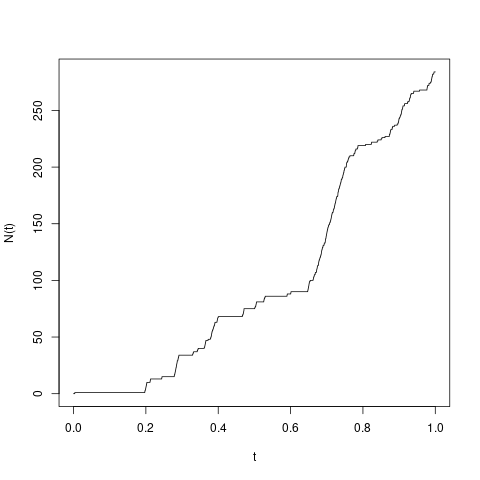
\includegraphics[width=.45\textwidth]{\figcp/FigSegPP-Chiroptere-seq2295-day2019-07-17-Path}
      \end{overprint}
    \end{tabular}
  \end{tabular}

  \bigskip
  \onslide+<3->{\paragraph{Intensity function $\lambda(t)$:} 
  $$
  \lambda(t) = \lim_{\Delta t \rightarrow 0} \frac{\Pbb\{N(t+\Delta t) - N(t) = 1\}}{\Delta t}, 
  \qquad \qquad 
  \Esp N(s) - \Esp N(t) = \int_t^s \lambda(u) \d u
  $$}
}

%====================================================================
\frame{\frametitle{Change-point detection} 

  \begin{tabular}{cc}
    \hspace{-.04\textwidth}
    \begin{tabular}{p{.45\textwidth}}
      \paragraph{Piecewise constant intensity function.} \\ ~ \\
      Change-points
      $$
      (\tau_0 =) 0 < \tau_1 \dots < \tau_{K-1} < 1 (= \tau_K)
      $$ \\
      
      For $t \in I_k = ]\tau_{k-1}, \tau_k]$:
      $$
      \lambda(t) = \lambda_k
      $$ \\
      
      \ra Continuous piece-wise linear cumulated intensity function      
    \end{tabular}
    & 
    \hspace{-.05\textwidth}
    \begin{tabular}{p{.45\textwidth}}
      \begin{overprint}
        \onslide<1>
        \paragraph{Bat cries} (night of the 17 jul. 2019)\footnote{source: Vigie-Chiro program, Y. Bas, CESCO-MNHN} \\
        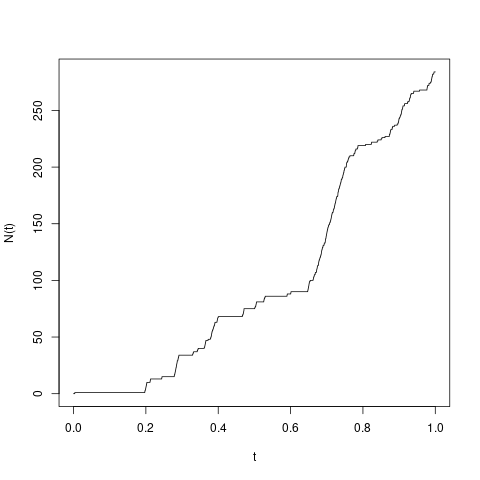
\includegraphics[width=.45\textwidth, trim=0 10 0 10, clip=]{\figcp/FigSegPP-Chiroptere-seq2295-day2019-07-17-Path}
        \onslide<2>
        \paragraph{Bat cries} (night of the 17 jul. 2019)\footnote{source: Vigie-Chiro program, Y. Bas, CESCO-MNHN} \\
        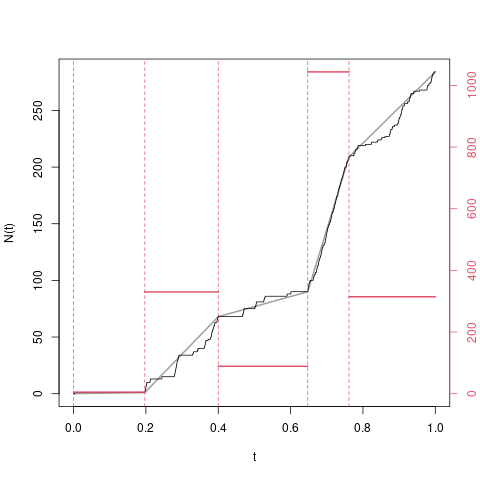
\includegraphics[width=.45\textwidth, trim=0 10 0 10, clip=]{\figcp/FigSegPP-Chiroptere-seq2295-day2019-07-17-Seg}
        \onslide<3>
        \paragraph{Kilauea eruptions} \\ ~ \\
        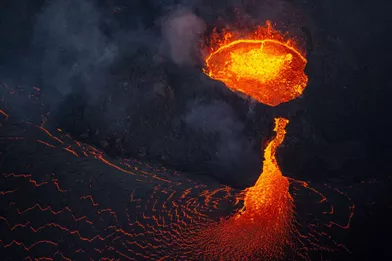
\includegraphics[width=.45\textwidth, height=.5\textheight]{\figcp/Kilauea-Wikipedia}
        \onslide<4>
        \paragraph{Kilauea eruptions} (from 1750 to 1984)\footnote{source: \refer{HoB17}} \\
        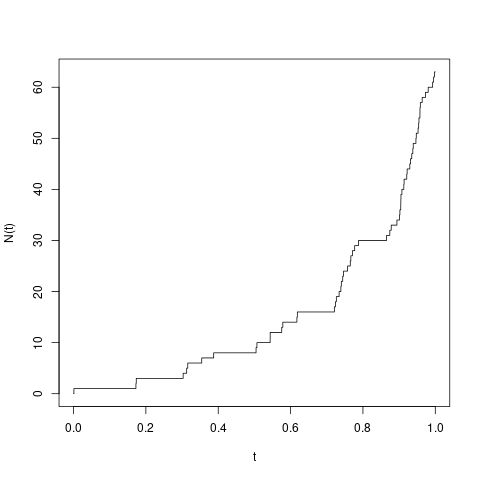
\includegraphics[width=.45\textwidth, trim=0 10 0 10, clip=]{\figcp/FigSegPP-Kilauea-Path}
        \onslide<5>
        \paragraph{Kilauea eruptions} (from 1750 to 1984)\footnote{source: \refer{HoB17}}  \\
        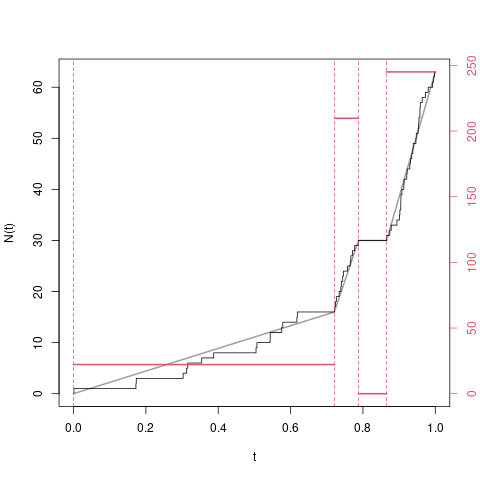
\includegraphics[width=.45\textwidth, trim=0 10 0 10, clip=]{\figcp/FigSegPP-Kilauea-Seg}
      \end{overprint}
    \end{tabular}
  \end{tabular}
  
  \bigskip \pause
  \paragraph{Aim.} 
  \begin{itemize}
   \item Segmentation: estimate $(\tau, \lambda)$ reasonnably fast 
   \item Model selection: choose $K$
  \end{itemize}
}

%====================================================================
%====================================================================
\section{Estimation}
\frame{\frametitle{Outline} \tableofcontents[currentsection]}
%====================================================================
\frame{\frametitle{Maximum-likelihood segmentation} 

  \paragraph{Property 1:} Independence of disjoint intervals.
  
  \bigskip \bigskip \pause
  \paragraph{Neg-log-likelihood.} Denoting $\dN_k = N(\tau_k) - N(\tau_{k-1})$, $\dtau_k = \tau_k - \tau_{k-1}$, 
  $$
  - \log p_{\tau, \lambda}(N) = \sum_{k=1}^K \lambda_k \dtau_k - \dN_k \log \lambda_k, 
%   \qquad \text{where} \quad
%   \left\{ \begin{array}{l}
%             \dN_k = N(\tau_k) - N(\tau_{k-1}), \\
%             \dtau_k = \tau_k - \tau_{k-1}
%           \end{array}\right.
  $$

  \bigskip \pause
  \paragraph{Additive contrast.} Sum over the segments
  $$
  \gamma(\tau, \lambda) = \sum_{k=1}^K C(\dN_k, \dtau_k, \lambda_k)
  $$

  \bigskip \pause
  \paragraph{Optimization problem.} 
  $$
  (\widehat{\tau}, \widehat{\lambda}) = \argmin_{\tau \in \Tcal^K} \; \min_{\lambda} \; \gamma(\tau, \lambda) 
  $$
  where $\Tcal^K$ is a {\sl continuous set}
%   :
%   $$
%   \Tcal = \left\{\tau \in [0, 1]^{K+1}: 0 = \tau_0 < \tau_1 \dots < \tau_{K-1} < \tau_K = 1\right\}
%   $$
  and $\gamma(\tau, \lambda)$ is {\sl not convex} nor even {\sl continuous}.
}

%====================================================================
\frame{\frametitle{Shape of the contrast fonction} 

  \begin{tabular}{cc}
    \hspace{-.04\textwidth}
    \begin{tabular}{p{.5\textwidth}}
      \paragraph{Optimization wrt $\lambda$:}
      $$
      \widehat{\gamma}(\tau) = \sum_{k=1}^K \underset{\widehat{C}(\dN_k, \dtau_k)}{\underbrace{C(\dN_k, \dtau_k, \emphase{\widehat{\lambda}_k})}}
      $$
      e.g.: $\widehat{\lambda}_k = \dN_k / \dtau_k$
    \end{tabular}
    & 
    \hspace{-.05\textwidth}
    \begin{tabular}{p{.5\textwidth}}
      \begin{overprint}
      \onslide<3>
      \hspace{-.07\textwidth}
      \includegraphics[width=.430\textwidth, height=.25\textheight]{\figcp/FigSegPPP-simul-n10-K1-seed1-Path}        
      \onslide<4>\includegraphics[width=.385\textwidth, height=.30\textheight]{\figcp/Turtle-FriendsOfTheSea}        
      \end{overprint}
    \end{tabular}
    \\
    \hspace{-.04\textwidth}
    \begin{tabular}{p{.5\textwidth}}
      \vspace{-0.05\textheight}
      \onslide+<2->{\paragraph{Optimization wrt $\tau$:}
      $$
      \widehat{\tau} = \argmin_\tau \widehat{\gamma}(\tau) = \sum_k \widehat{C}(\dN_k, \dtau_k)
      $$}
      ~ \\ 
      \bigskip 
      \onslide+<3->{
      \paragraph{Example:} $n = 10$, $K=3$. ~\\
      Each block corresponds to a specific vector
      $$
      \dN = (\dN_1, \dN_2, \dN_3)
      $$
      }
    \end{tabular}
    & 
    \hspace{-.65\textwidth}
    \begin{tabular}{p{.5\textwidth}}
      \vspace{-0.05\textheight}
      \onslide<3->{\includegraphics[width=.45\textwidth, trim=0 0 20 50, clip=]{\figcp/FigSegPPP-simul-n10-K1-seed1-Contrast}}  
    \end{tabular}
  \end{tabular}

}

%====================================================================
\frame{\frametitle{Partitioning the segmentation space} 

  \paragraph{Partitioning the number of events.} Define
  $
  \Ncal^K = \left\{\nu \in \Nbb^K: \sum_{k=1}^K \nu_k = n\right\}.
  $

  \bigskip \bigskip \pause
  \paragraph{Partitioning the segmentation space.} For $\nu \in \Ncal_K$, define
  $
  \Tcal^K_\nu = \left\{\tau \in \Tcal^K: \dN = \nu\right\}
  $
  so that
  $$
  \min_{\tau \in \Tcal^K} \widehat{\gamma}(\tau) 
  = \min_{\nu \in \Ncal^K} \min_{\tau \in \Tcal^K_\nu} \widehat{\gamma}(\tau, ).
  $$

  \bigskip \pause
  \paragraph{Property.} If $K\leq n$ and, for each $\nu \in \Ncal^K$, 
  $\widehat{\gamma}(\tau)$ is \emphase{strictly concave wrt} $\tau \in \Tcal^K_\nu$, then
  $$
  \widehat{\tau} = \argmin_{\tau \in \Tcal^K} \widehat{\gamma}(\tau) 
  \subset \{T_1^-, T_1, T_2^-, T_2^-, \dots T_n^-, T_n\}.
  $$

  \bigskip \pause
  \paragraph{Consequence.} $\widehat{\tau}$ can be obtained by dynamic programming over the $2n+2$ possible change-points 
  $$
  \Scal = \{0, T_1^-, T_1, T_2^-, T_2, \dots T_n^-, T_n, 1\}.
  $$
}


%====================================================================
\frame{\frametitle{Alternative constrast} 

  \paragraph{Remark.} 
  \begin{itemize}
   \item $\Scal$ includes segments with length 0 (e.g.: $I = ]T_k^-, T_k]$, $\dN_k = 1$), 
   \item ... which are optimal for the log-likelihood contrast: $\widehat{C}(1, 0) = -\infty$
  \end{itemize}
  
  \bigskip \bigskip \pause
%   \paragraph{Alternative models/contrasts.} For each segment $1 \leq k \leq K$
%   \begin{description}
%     \item[Gamma + Poisson:] $\lambda_k & \sim \Gam(a, b)$, $\{N(t)\}_{t \in I_k} \mid \lambda_k \sim PP(\lambda_k)$
%     \begin{align*}
%     C(\dN_k, \dtau_k, \lambda_k) & = \log p_{a, b}(\lambda_k, \{N(t)\}_{t \in I_k}) \\
% %     & = \cst - (a + \dN_k - 1)\log \lambda_k + (b+\dtau_k) \lambda_k \\
%     \Rightarrow \qquad
%     \widehat{C}(\dN_k, \dtau_k) 
%     & = \cst + (a + \dN_k - 1) \left(1 - \log\left(\frac{a + \dN_k - 1}{b+\dtau_k}\right)\right)
%     \end{align*}
%     \item[Poisson-Gamma:] \pause same model but
%     \begin{align*}
%     C(\dN_k, \dtau_k) & = \log p_{a, b}(\{N(t)\}_{t \in I_k}) \\
%     & = \cst - \log \Gamma(a + \dN_k) + (a + \dN_k) \log(b + \dtau_k)
%     \end{align*}
%   \end{description}
  \paragraph{Poisson-Gamma model.} For each segment $1 \leq k \leq K$:
  $$
  \Lambda_k \sim \Gam(a, b), \qquad \qquad
  \{N(t)\}_{t \in I_k} \mid \Lambda_k \sim PP(\Lambda_k),
  $$
  which gives:
  \begin{align*}
  C(\dN_k, \dtau_k) & = - \log p_{a, b}(\{N(t)\}_{t \in I_k}) \\
  & = \cst - \log \Gamma(a + \dN_k) + (a + \dN_k) \log(b + \dtau_k)
  \end{align*}

  \bigskip
  \ra Enjoys the concavity property, but avoids segments with null length.

}

%====================================================================
%====================================================================
\section{Model selection}
\frame{\frametitle{Outline} \tableofcontents[currentsection]}
%====================================================================
\frame{\frametitle{Model selection} 

  \paragraph{Property 2: Thining.} ~ \\
%   \begin{itemize}
%     \item Let $\{N(t)\}_{0 \leq t \leq 1} \sim PP(\lambda(t))$ with event times $T_1 < \dots < T_n$, 
%     \item Randomly assign each event time to set $L$ (with prob. $v$) or $T$ (with prob. $1-v$), 
%     \item Set $\{T_i\}_{i \in L}$ (resp $T$) as the event times of $\{N^L(t)\}_{0 \leq t \leq 1}$ (resp. $\{N^T(t)\}$)
%     \item \pause Then:
%     $$
%     \{N^L(t)\} \sim PP(\lambda^L(t)), \qquad 
%     \{N^T(t)\} \sim PP(\lambda^T(t))
%     $$
%     and
%     $$
%     \lambda^L(t) = v \lambda(t), \qquad
%     \lambda^T(t) = (1-v) \lambda(t), \qquad
%     \{N^L(t)\} \perp \{N^T(t)\}.
%     $$
%   \end{itemize}
  \begin{tabular}{cc}
    \hspace{-.04\textwidth}
    \begin{tabular}{p{.5\textwidth}}
      \begin{itemize}
       \item $\{N(t)\} \sim PP(\lambda(t))$
       \item Sample the event times (prob. $v$) 
      \end{itemize}
    \end{tabular}
    & 
    \hspace{-.15\textwidth}
    \begin{tabular}{p{.4\textwidth}}
      \begin{overprint}
        \onslide<1>
        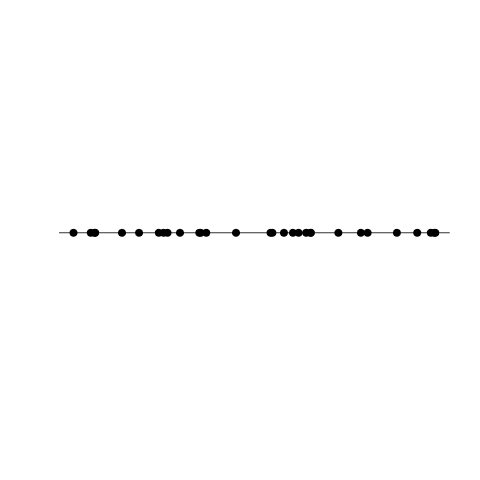
\includegraphics[width=.5\textwidth, trim=0 225 0 225, clip=]{\figcp/FigSegPP-ThiningOriginal.png}
        \onslide<2->
        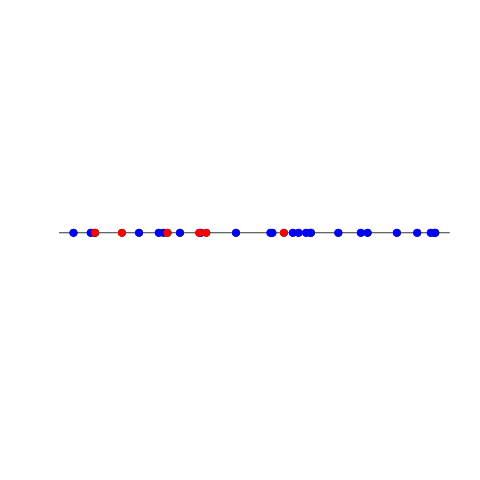
\includegraphics[width=.5\textwidth, trim=0 225 0 225, clip=]{\figcp/FigSegPP-ThiningSampling.png}
      \end{overprint}
    \end{tabular}
  \end{tabular}
  \pause
  $$
  \textcolor{blue}{\{N^L(t)\}} \sim PP(v\lambda(t)), \qquad
  \textcolor{red}{\{N^T(t)\}} \sim PP((1-v)\lambda(t)), \qquad
  {\{N^L(t)\}} \perp {\{N^T(t)\}}
  $$
  
  \bigskip \bigskip \pause
  \paragraph{Consequence.} If $\lambda(t)$ is piece-wise constant with parms $\tau = (\tau_k)$ and $\lambda = (\lambda_k)$, then \pause
  \begin{itemize}
   \item $\lambda^L(t)$ piece-wise constant with change points $(\tau_k)$ and intensities $(v \lambda_k)$, 
   \item $\lambda^T(t)$ piece-wise constant with change points $(\tau_k)$ and intensities $((1-v) \lambda_k)$, 
   \item $\{N^L(t)\} \perp \{N^T(t)\}$.
  \end{itemize}
}

%====================================================================
\frame{\frametitle{Cross validation} 

  Sampling event times provides two independent Poisson processes with \emphase{same change points}.
  
  \bigskip \bigskip \pause
  \paragraph{Cross-validation.} For $1 \leq K \leq K_{\max}$, 
  \begin{itemize}
   \item Repeat for $1 \leq m \leq M$ : \\
      \medskip
      1 -- Sample the event times to form $\{N^{L, m}(t)\}$ (\emphase{learn}) and $\{N^{T, m}(t)\}$ (\emphase{test}), \\
      \medskip
      2 -- Estimate $\widehat{\tau}^{L, m}$ and $\widehat{\lambda}^{L, m}$ from $\{N^{L, m}(t)\}$, \\
      \medskip
      3 -- Compute the contrast $\displaystyle{\gamma_K^{T, m} = \gamma\left(\{N^T(t)\}; \widehat{\tau}^{L, m}, \emphase{\frac{1-v}{v}}\widehat{\lambda}^{L, m}\right)}$.
    \bigskip
    \item \pause Compute
    $$
    \overline{\gamma}_K = \frac1M \sum_{m=1}^M \gamma_K^{T, m}
    $$
    \medskip
    \item \pause Select
    $$
    \widehat{K} = \argmin_K \overline{\gamma}_K
    $$
  \end{itemize}
}

%====================================================================
\frame{\frametitle{Illustration} 

  \bigskip
  \paragraph{Poisson-Gamma contrast.}
  Set $a^L = a^T = 1$, $b^L = 1/n_L$, $b^T = 1/n_T$, and compute
  \begin{align*}
    - \log p(\{N^T(t)\} \mid \widehat{\tau}^L) 
    & = \sum_{k=1}^K (a + \dN_k^T) \log(a + \dtau_k) - \log \Gamma(a + \dN_k^L) \\
    & \quad - K \left(a^T \log b^T - \log \Gamma(a^T)\right)
  \end{align*}

  \bigskip \bigskip \pause
  \paragraph{Kilauea eruptions} \\
  \begin{tabular}{cc}
    \hspace{-.04\textwidth}
    \begin{tabular}{p{.45\textwidth}}
      Model selection via CV \\
      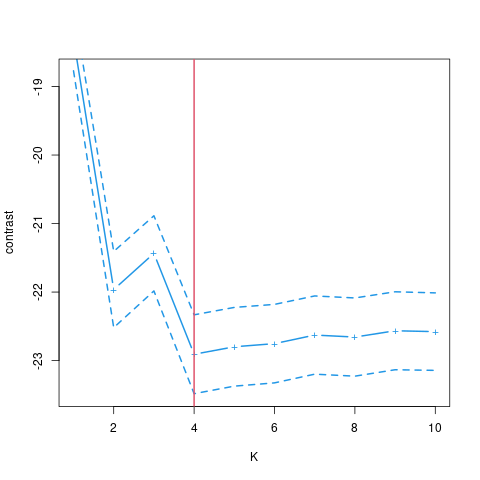
\includegraphics[width=.4\textwidth, trim=0 10 10 10, clip=]{\figcp/FigSegPP-Kilauea-CV-PGtrain}
    \end{tabular}
    & 
    \hspace{-.05\textwidth}
    \begin{tabular}{p{.45\textwidth}}
      Resulting segmentation \\
      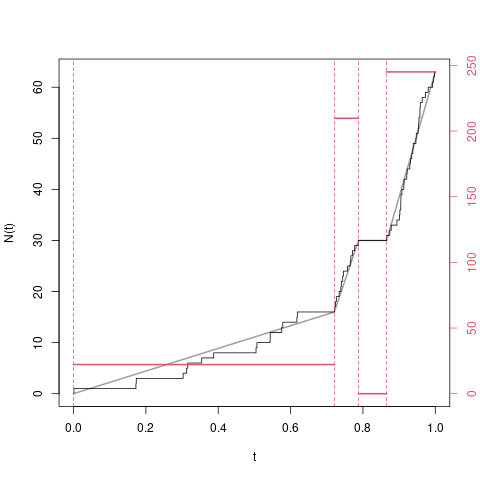
\includegraphics[width=.4\textwidth, trim=0 10 0 10, clip=]{\figcp/FigSegPP-Kilauea-Seg}
    \end{tabular}
  \end{tabular}

}

%====================================================================
%====================================================================
\section{Extensions}
\frame{\frametitle{Outline} \tableofcontents[currentsection]}
%====================================================================
\frame{\frametitle{Extensions} 

  \paragraph{Marked Poisson Process.}
  \begin{itemize}
    \item $\{Y(t)\}_{0 \leq t \leq 1} \sim MPP(\lambda(t), \mu(t))$:
    $$
    \{N(t)\}_{0 \leq t \leq 1} \sim PP(\lambda(t)), \qquad
    \text{at each $T_i$:} \quad X_i \sim \Fcal(\mu(T_i))
    $$
    \item Works the same way, provided that concavity holds.
    \item Bat cries: $X =$ bat species or cry duration.
  \end{itemize}
  
  \bigskip \bigskip \pause
  \paragraph{Segmentation-clustering.}
  \begin{itemize}
    \item Each segment belongs to a class $1 \leq q \leq Q$ (with probability $\pi_q$ and intensity $\lambda_k = \ell_q$), 
    \item Combination of EM and DP algorithms \refer{PRL07}, 
    \item Class = animal behaviour (hunt, transit, ...)
  \end{itemize}

  \bigskip \bigskip \pause
  \paragraph{And also.}
  \begin{itemize}
    \item Theoretically grounded model selection criterion, 
    \item Other desirable contrasts, ...
  \end{itemize}
}

%====================================================================
\frame[allowframebreaks]{ \frametitle{References}
  {
   \tiny
   \bibliography{/home/robin/Biblio/BibGene}
   \bibliographystyle{alpha}
  }
}

%====================================================================
\frame{\frametitle{Appendix} 

  $$
  |\Ncal_K| = \sum_{h=\lfloor (K-1)/2\rfloor}^K {{n-1}\choose{h-1}} {{h+1}\choose{K-h}}
  $$

}

%====================================================================
\backupbegin
%====================================================================


%====================================================================
\backupend
%====================================================================

%====================================================================
%====================================================================
\end{document}
%====================================================================
%====================================================================
  
  \begin{tabular}{cc}
    \hspace{-.04\textwidth}
    \begin{tabular}{p{.5\textwidth}}
    \end{tabular}
    & 
    \hspace{-.02\textwidth}
    \begin{tabular}{p{.5\textwidth}}
    \end{tabular}
  \end{tabular}

